% \subsection{Stuff}

% Fig. \ref{fig:lift_drag} shows the lift and drag time evolution, and Fig. \ref{fig:lift_drag_u} the lift and drag steady states converged  as functions of velocity.


% \begin{figure}[ht!]
%     \centering
%     \begin{subfigure}{0.48\textwidth}
%         \begin{tikzpicture}
%             \begin{axis}[
%                 xmin=0, xmax=6,
%                 ymin=0.3e5, ymax=0.8e5,
%                 legend pos=north east,
%                 xlabel = {t (s)},
%                 ylabel = {Lift (N)},
%                 no markers,
%                 every axis plot/.append style={ultra thick},
%                 width=0.98\textwidth, 
%                 ]
%                 \addplot +[mark=none, color=\firstcolor, style=solid] table[y expr=\thisrowno{3}] {curves/fixed/force_3.dat};
%                 \addplot +[mark=none, color=\secondcolor, style=solid] table[y expr=\thisrowno{3}] {curves/fixed/force_5.dat};
%                 \addplot +[mark=none, color=\thirdcolor, style=solid] table[y expr=\thisrowno{3}] {curves/fixed/force_7.dat};
%                 \addplot +[mark=none, color=\fourthcolor, style=solid] table[y expr=\thisrowno{3}] {curves/fixed/force_9.dat};
%                 \addplot +[mark=none, color=\fifthcolor, style=solid] table[y expr=\thisrowno{3}] {curves/fixed/force_11.dat};
%                 \addplot +[mark=none, color=\sixthcolor, style=solid] table[y expr=\thisrowno{3}] {curves/fixed/force_13.dat};
%                 \addplot +[mark=none, color=\seventhcolor, style=solid] table[y expr=\thisrowno{3}] {curves/fixed/force_15.dat};
%             \end{axis} 
%         \end{tikzpicture}   
%         \caption{Lift evolution.}
%         \label{fig:lift}
%     \end{subfigure}
%     \begin{subfigure}{0.48\textwidth}
%         \begin{tikzpicture}
%             \begin{axis}[
%                 xmin=0, xmax=6,
%                 ymin=0, ymax=2e4,
%                 legend pos=north east,
%                 xlabel = {t (s)},
%                 ylabel = {Drag (N)},
%                 no markers,
%                 every axis plot/.append style={ultra thick},
%                 width=0.98\textwidth, 
%                 ]
%                 \addplot +[mark=none, color=\firstcolor, style=solid] table[y expr=-\thisrowno{1}] {curves/fixed/force_3.dat};
%                 \addplot +[mark=none, color=\secondcolor, style=solid] table[y expr=-\thisrowno{1}] {curves/fixed/force_5.dat};
%                 \addplot +[mark=none, color=\thirdcolor, style=solid] table[y expr=-\thisrowno{1}] {curves/fixed/force_7.dat};
%                 \addplot +[mark=none, color=\fourthcolor, style=solid] table[y expr=-\thisrowno{1}] {curves/fixed/force_9.dat};
%                 \addplot +[mark=none, color=\fifthcolor, style=solid] table[y expr=-\thisrowno{1}] {curves/fixed/force_11.dat};
%                 \addplot +[mark=none, color=\sixthcolor, style=solid] table[y expr=-\thisrowno{1}] {curves/fixed/force_13.dat};
%                 \addplot +[mark=none, color=\seventhcolor, style=solid] table[y expr=-\thisrowno{1}] {curves/fixed/force_15.dat};
%             \end{axis}
%         \end{tikzpicture}   
%         \caption{Drag evolution.}
%         \label{fig:drag}
%     \end{subfigure}

%     \begin{tikzpicture}
%         \begin{axis}[
%             hide axis,
%             xmin=0, xmax=1, ymin=0, ymax=1,
%             legend columns=3, % -1 pour aligner horizontalement, 1 pour aligner verticalement
%             legend entries={$u=3$, $u=5$, $u=7$, $u=9$, $u=11$, $u=13$, $u=15$},
%             % cycle list/Set2-8,
%             width=0.25\textwidth
%         ]
%         \addlegendimage{ultra thick, \firstcolor}
%         \addlegendimage{ultra thick, \secondcolor}
%         \addlegendimage{ultra thick, \thirdcolor}
%         \addlegendimage{ultra thick, \fourthcolor}
%         \addlegendimage{ultra thick, \fifthcolor}
%         \addlegendimage{ultra thick, \sixthcolor}
%         \addlegendimage{ultra thick, \seventhcolor}
%         \end{axis}
%     \end{tikzpicture}
%     \caption{Lift and drag evolution - fixed boat.}
%     \label{fig:lift_drag}
% \end{figure}



% \begin{figure}[ht!]
%     \centering
%     \begin{subfigure}{0.48\textwidth}
%         \begin{tikzpicture}
%             \begin{axis}[
%                 xmin=0, xmax=15,
%                 ymin=0.3e5, ymax=0.8e5,
%                 legend pos=north east,
%                 xlabel = {u (m/s)},
%                 ylabel = {Lift (N)},
%                 every axis plot/.append style={ultra thick},
%                 width=0.98\textwidth, 
%                 ]
%                 \addplot +[mark=*, mark options={fill=\firstcolor}, color=\firstcolor, style=solid] table[y expr=\thisrowno{1}] {curves/fixed/force_speed};
%                 \addplot +[mark=*, mark options={fill=\firstcolor}, color=\firstcolor, style=dotted] table[y expr=\thisrowno{1}] {curves/fixed/force_nofoil_speed};
%             \end{axis} 
%         \end{tikzpicture}   
%         \caption{Lift evolution.}
%         \label{fig:lift_u}
%     \end{subfigure}
%     \begin{subfigure}{0.48\textwidth}
%         \begin{tikzpicture}
%             \begin{axis}[
%                 xmin=0, xmax=15,
%                 ymin=0, ymax=3e4,
%                 legend pos=north east,
%                 xlabel = {u (m/s)},
%                 ylabel = {Drag (N)},
%                 every axis plot/.append style={ultra thick},
%                 width=0.98\textwidth, 
%                 ]
%                 \addplot +[mark=*, mark options={fill=\firstcolor}, color=\firstcolor, style=solid] table[y expr=\thisrowno{2}] {curves/fixed/force_speed};
%                 \addplot +[mark=*, mark options={fill=\firstcolor}, color=\firstcolor, style=dotted] table[y expr=\thisrowno{2}] {curves/fixed/force_nofoil_speed};
%             \end{axis}
%         \end{tikzpicture}   
%         \caption{Drag evolution.}
%         \label{fig:drag_u}
%     \end{subfigure}
%     \begin{tikzpicture}
%         \begin{axis}[
%             hide axis,
%             xmin=0, xmax=1, ymin=0, ymax=1,
%             legend columns=3, % -1 pour aligner horizontalement, 1 pour aligner verticalement
%             legend entries={hull and foil, hull only},
%             % cycle list/Set2-8,
%             width=0.25\textwidth
%         ]
%         \addlegendimage{ultra thick, mark=*, mark options={fill=\firstcolor}, solid, \firstcolor}
%         \addlegendimage{ultra thick, mark=*, mark options={fill=\firstcolor}, dotted, \firstcolor}
%         \end{axis}
%     \end{tikzpicture}
%     \caption{Lift and drag evolution - fixed boat.}
%     \label{fig:lift_drag_u}
% \end{figure}


\subsection{Force time evolution and mesh convergence}

    \begin{figure}[ht!]
        \centering
        \begin{subfigure}{0.48\textwidth}
            \begin{tikzpicture}
                \begin{axis}[
                    xlabel={time (s)},
                    ylabel={Lift (N)},
                    % xmin=0, xmax=1e4, 
                    % ymin=1.3e4, ymax=1.5e4,
                    ymajorgrids=true,xmajorgrids=true,
                    legend pos=south east,
                    width=0.98\textwidth,
                    axis background/.style={fill=\backgroundcolor}
                    ]
                    \addplot +[mark=None, style=ultra thick, color=\firstcolor, style=ultra thick, style=solid] table[x expr=(\thisrowno{0}), y expr=(\thisrowno{3})] {curves/forces/force_200k};
                    \addplot +[mark=None, style=ultra thick, color=\secondcolor, style=ultra thick, style=solid] table[x expr=(\thisrowno{0}), y expr=(\thisrowno{3})] {curves/forces/force_300k};
                    \addplot +[mark=None, style=ultra thick, color=\thirdcolor, style=ultra thick, style=solid] table[x expr=(\thisrowno{0}), y expr=(\thisrowno{3})] {curves/forces/force_200k_nofoils};
                \end{axis}
            \end{tikzpicture}
            \caption{Lift evolution.}
            \label{fig:lift_evolution}
        \end{subfigure}
        \begin{subfigure}{0.48\textwidth}
            \begin{tikzpicture}
                \begin{axis}[
                    xlabel={time (s)},
                    ylabel={Drag (N)},
                    % xmin=0, xmax=20000,
                    % ymin=3.7e3, ymax=4.5e3,
                    ymajorgrids=true,xmajorgrids=true,
                    legend pos=south east,
                    width=0.98\textwidth,
                    axis background/.style={fill=\backgroundcolor}
                    ]
                    \addplot +[mark=None, style=ultra thick, color=\firstcolor, style=ultra thick, style=solid] table[x expr=(\thisrowno{0}), y expr=(-\thisrowno{1})] {curves/forces/force_200k};
                    \addplot +[mark=None, style=ultra thick, color=\secondcolor, style=ultra thick, style=solid] table[x expr=(\thisrowno{0}), y expr=(-\thisrowno{1})] {curves/forces/force_300k};
                    \addplot +[mark=None, style=ultra thick, color=\thirdcolor, style=ultra thick, style=solid] table[x expr=(\thisrowno{0}), y expr=(-\thisrowno{1})] {curves/forces/force_200k_nofoils};
                \end{axis}
            \end{tikzpicture}
            \caption{Drag evolution.}
            \label{fig:drag_evolution}
        \end{subfigure}
        \begin{subfigure}{0.48\textwidth}
            \begin{tikzpicture}
                \begin{axis}[
                    xlabel={time (s)},
                    ylabel={z (m)},
                    % xmin=0, xmax=20000,
                    % ymin=3.7e3, ymax=4.5e3,
                    ymajorgrids=true,xmajorgrids=true,
                    legend pos=south east,
                    width=0.98\textwidth,
                    axis background/.style={fill=\backgroundcolor}
                    ]
                    \addplot +[mark=None, style=ultra thick, color=\firstcolor, style=ultra thick, style=solid] table[x expr=(\thisrowno{0}), y expr=(\thisrowno{3})] {curves/rigidBodyMotionDisplacement/tq_200k};
                    \addplot +[mark=None, style=ultra thick, color=\secondcolor, style=ultra thick, style=solid] table[x expr=(\thisrowno{0}), y expr=(\thisrowno{3})] {curves/rigidBodyMotionDisplacement/tq_300k};
                    \addplot +[mark=None, style=ultra thick, color=\thirdcolor, style=ultra thick, style=solid] table[x expr=(\thisrowno{0}), y expr=(\thisrowno{3})] {curves/rigidBodyMotionDisplacement/tq_200k_nofoils};
                \end{axis}
            \end{tikzpicture}
            \caption{Vertical displacement evolution.}
            \label{fig:drag_evolution}
        \end{subfigure}
        
        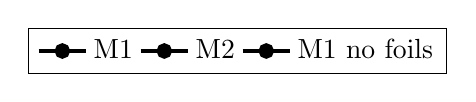
\begin{tikzpicture}
            \begin{axis}[
                hide axis,
                xmin=0, xmax=1, ymin=0, ymax=1,
                legend columns=-1, % -1 pour aligner horizontalement, 1 pour aligner verticalement
                legend entries={M1, M2, M1 no foils},
                width=0.25\textwidth
                ]
                \addlegendimage{ultra thick, mark=*, \firstcolor}
                \addlegendimage{ultra thick, mark=*, \secondcolor}
                \addlegendimage{ultra thick, mark=*, \thirdcolor}
            \end{axis}
        \end{tikzpicture}

        \caption{Convergence of the metrics with the iterations.}
        \label{fig:meshConvergence}
    \end{figure}

    

    % \begin{figure}[ht!]
    %     \centering
    %     \begin{subfigure}{0.3\textwidth}
    %         \begin{tikzpicture}
    %             \begin{axis}[
    %                 % xlabel={mesh},
    %                 % ylabel={Lift},
    %                 % xmin=0, xmax=1e4, 
    %                 % ymin=1.3e4, ymax=1.5e4,
    %                 ymajorgrids=true,xmajorgrids=true,
    %                 legend pos=south east,
    %                 width=0.98\textwidth,
    %                 % title={z},
    %                 width=0.98\textwidth,
    %                 axis background/.style={fill=\backgroundcolor}
    %                 ]
    %                 \addplot +[mark=None, style=ultra thick, color=\firstcolor, style=ultra thick, style=solid] table[x expr=(\thisrowno{0}), y expr=(\thisrowno{1})] {curves/convergence/meshConvergence};
    %             \end{axis}
    %         \end{tikzpicture}
    %         \caption{Displacement (m).}
    %         \label{fig:lift_evolution}
    %     \end{subfigure}
    %     \begin{subfigure}{0.3\textwidth}
    %         \begin{tikzpicture}
    %             \begin{axis}[
    %                 % xlabel={time},
    %                 % ylabel={Drag},
    %                 % xmin=0, xmax=20000,
    %                 % title={Lift},
    %                 width=0.98\textwidth,
    %                 % ymin=3.7e3, ymax=4.5e3,
    %                 ymajorgrids=true,xmajorgrids=true,
    %                 legend pos=south east,
    %                 width=0.98\textwidth,
    %                 axis background/.style={fill=\backgroundcolor}
    %                 ]
    %                 \addplot +[mark=None, style=ultra thick, color=\firstcolor, style=ultra thick, style=solid] table[x expr=(\thisrowno{0}), y expr=(\thisrowno{2})] {curves/convergence/meshConvergence};
    %             \end{axis}
    %         \end{tikzpicture}
    %         \caption{Lift (N).}
    %         \label{fig:drag_evolution}
    %     \end{subfigure}
    %     \begin{subfigure}{0.3\textwidth}
    %         \begin{tikzpicture}
    %             \begin{axis}[
    %                 % xlabel={time},
    %                 % ylabel={elevation},
    %                 % xmin=0, xmax=20000,
    %                 % title={Drag},
    %                 width=0.98\textwidth,
    %                 % ymin=3.7e3, ymax=4.5e3,
    %                 ymajorgrids=true,xmajorgrids=true,
    %                 legend pos=south east,
    %                 width=0.98\textwidth,
    %                 axis background/.style={fill=\backgroundcolor}
    %                 ]
    %                 \addplot +[mark=None, style=ultra thick, color=\firstcolor, style=ultra thick, style=solid] table[x expr=(\thisrowno{0}), y expr=(\thisrowno{3})] {curves/convergence/meshConvergence};
    %             \end{axis}
    %         \end{tikzpicture}
    %         \caption{Drag (N).}
    %         \label{fig:drag_evolution}
    %     \end{subfigure}
    %     \caption{.}
    %     \label{fig:meshConvergence}
    % \end{figure}

